%%% IEEE 系学会向け LaTeX テンプレート
\documentclass[10pt,conference,a4paper,nofonttune]{IEEEtran}
%!TEX encoding = UTF-8 Unicode
%
% 卒論 / 修論用 プリアンブル
%

%% フォント
\usepackage{lmodern}
\usepackage[scale=0.95]{tgheros}
\usepackage{textcomp}
\usepackage[scaled=0.85]{beramono}
\usepackage[T1]{fontenc}

%% パッケージ
\usepackage[cmex10]{amsmath}
\usepackage{amssymb,amsfonts,mathtools,bm}

\usepackage{graphicx,color}
\usepackage[table]{xcolor}

\usepackage[pdfborder={0 0 0}]{hyperref}
\usepackage{pxjahyper}

% caption のコロン「図4.4: キャプション」を「図4.4 キャプション」に直す
\usepackage[labelsep=quad,compatibility=false]{caption}
\usepackage[belowskip=1.2em]{subcaption}

\usepackage{cite,url,array,makecell}
\usepackage{algorithm,algorithmic}

% 数学コマンドの補完
\DeclareMathOperator*{\sinc}{sinc}
\DeclareMathOperator*{\prox}{prox}
\DeclareMathOperator*{\argmin}{argmin}
\DeclareMathOperator*{\argmax}{argmax}

% 参考文献表示スタイルを変更
\bibliographystyle{sieicej}

% 赤色を少し暗くする
\definecolor{red}{rgb}{0.75,0,0}

\makeatletter
   % アルゴリズム図キャプションの表記を「Algorithm」→「アルゴリズム」に
   \renewcommand{\ALG@name}{アルゴリズム}
\makeatother

% 修正箇所に色付けするコマンド
%
% ・ コマンド版
%   \fixed{修正箇所}
%
% ・ 環境版
%   \begin{fixedregion}
%      修正箇所
%   \end{fixedregion}
\newcommand{\fixed}[1]{#1} 
\newenvironment{fixedregion}{\ignorespaces}{\ignorespacesafterend}
% 下の 2 行をコメントアウトすることで色付けを無効化します
\renewcommand{\fixed}[1]{\textcolor{red}{#1}}
\renewenvironment{fixedregion}{\protect\leavevmode\color{red}\ignorespaces}{\ignorespacesafterend}

% 強調
\newcommand{\strong}[1]{\textcolor{red}{\textbf{#1}}}



%% \title : 一般の LaTeX 文書と同じ
%% IEEE スタイルでは各単語の頭を大文字にする (前置詞とかを除いて)
\title{Bare Demo of IEEEtran.cls for IEEE Conferences}

%% \author : 以下の様に組む
%  +--------------------------+
%  |  IEEEauthorblockN (名前)  |
%  +--------------------------+
%  |  IEEEauthorblockA (所属)  |
%  +--------------------------+
\author{\IEEEauthorblockN{Takanori Fujisawa, Masaaki Ikehara}
\IEEEauthorblockA{EEE Dept., Keio Univ., Yokohama, Kanagawa 223-8522, Japan\\
Email: \texttt{\url{{fujisawa,ikehara}@tkhm.elec.keio.ac.jp}}}}

\begin{document}

\maketitle

%% 概要
\begin{abstract}
Abstract goes here.
\lipsum[1]
\end{abstract}

%% IEEE Conference ではキーワードは入れない

%% 著作権表示 (文章の左下)
%% 学会名・著作権表示は学会によって変わります.
%% 学会の Web ページを見て正しいフォーマットに変更してください.
%% 著作権表示の指示がない or 分からない場合は
%% \begin{figure} ... \end{figure} までを削除してください.
\begin{figure}[!b]
   % 学会名
   \emph{International Workshop on Advanced Image Technology 2018 (IWAIT 2018),
   Jan. 7--10, 2018, Chiang Mai, Thailand.} \par
   % 著作権表示
   \emph{978-1-5386-2615-3/18/\$31.00 \ \copyright 2018 IEEE.}
\end{figure}

\section{Introduction}
This demo file is intended to serve as a ``starter file''
for IEEE conference papers produced under \LaTeX\ using
IEEEtran.cls version 1.8b and later.
% You must have at least 2 lines in the paragraph with the drop letter
% (should never be an issue)
I wish you the best of success.
% 引用は複数まとめて \cite に入れられる
\cite{IEEEexample:article_typical,IEEEexample:articleetal}

\lipsum[1]

\subsection{Subsection Heading Here}
Subsection text here.
\lipsum[2]

\subsubsection{Subsubsection Heading Here}
Subsubsection text here.


\section{Examples of Figures and Tables}
Fig.~\ref{fig:example} shows the result of ...
\lipsum[3-4]

%% 図の入れ方
\begin{figure}[t]
   % figure は t を指定する
   \centering
   % 横幅の 0.45 倍の minipage を 2x2 に配置
   %  [minipage][minipage]
   %  [1emの縦スペース]
   %  [minipage][minipage]
   \begin{minipage}{.45\hsize}
      \centering
      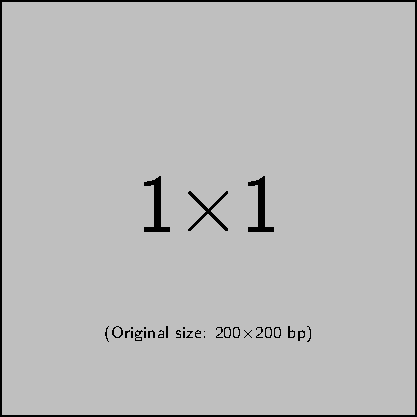
\includegraphics[width=.8\hsize]{figure/example-image-1x1.pdf} %
      \subcaption{Example Image A}
   \end{minipage}
   \begin{minipage}{.45\hsize} 
      \centering
      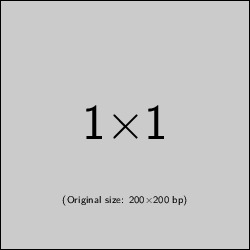
\includegraphics[width=.8\hsize]{figure/example-image-1x1.jpg} %
      \subcaption{Example Image B}
   \end{minipage}
   \\ \vspace{1em}
   \begin{minipage}{.45\hsize} 
      \centering
      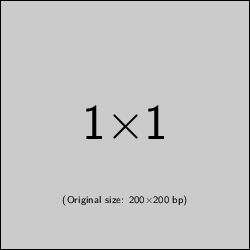
\includegraphics[width=.8\hsize]{figure/example-image-1x1.png} %
      \subcaption{Example Image C}
   \end{minipage}
   \begin{minipage}{.45\hsize} 
      \centering
      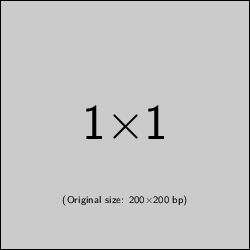
\includegraphics[width=.8\hsize]{figure/example-image-1x1.png} %
      \subcaption{Example Image D}
   \end{minipage}
   \caption{An Example of a Figure}
   \label{fig:example}
\end{figure}

%% 表の入れ方
\begin{table}[!t] \centering
   \caption{An Example of a Table}
   \label{Tbl:Example}
   {
      % 収まりきらないことが多いと思うので文字を小さくする
      % \footnotesize < \small < \normalsize (指定なし)
      \footnotesize
      %% 行間を 1.2 倍に広げる
      \renewcommand{\arraystretch}{1.2}
      \begin{tabular}{c|c|c|c|c|c|c}
\hline\hline
        & \multicolumn{6}{c}{Number of Occurences} \\\cline{2-7}
        & 0 & 1 & 2 & 3 & 4 & 5 and more \\\hline
Scheme 1&\texttt{10}&\texttt{11} &\multicolumn{4}{c}{\scriptsize Flag 0} \\\hline
Scheme 2&\texttt{10}&\texttt{110}&\texttt{111} &\multicolumn{3}{c}{\scriptsize Flag 0}\\\hline
Scheme 3&\texttt{10}&\texttt{110}&\texttt{1110}&\texttt{1111} &\multicolumn{2}{c}{\scriptsize Flag 0} \\\hline
Scheme 4&\texttt{10}&\texttt{110}&\texttt{1110}&\texttt{11110}&\texttt{11111}&{\scriptsize Flag 0}\\\hline
\hline
      \end{tabular}
   }
\end{table}

%% 表の入れ方2
\begin{table}[!t]
   \centering
   \caption{An Example of a Table with Subcaption}
   \label{Tbl:ExampleWithSubcaption}
   % 収まりきらないことが多いと思うので文字を小さくする
   % \footnotesize < \small < \normalsize (指定なし)
   \footnotesize
   %
   \subcaption{The first item}
   {
      \renewcommand{\arraystretch}{1.2}
      \begin{tabular}{c|c|c|c|c|c|c}
\hline\hline
        & \multicolumn{6}{c}{Number of Occurences} \\\cline{2-7}
        & 0 & 1 & 2 & 3 & 4 & 5 and more \\\hline
Scheme 1&\texttt{10}&\texttt{11} &\multicolumn{4}{c}{\scriptsize Flag 0} \\\hline
Scheme 2&\texttt{10}&\texttt{110}&\texttt{111} &\multicolumn{3}{c}{\scriptsize Flag 0}\\\hline
Scheme 3&\texttt{10}&\texttt{110}&\texttt{1110}&\texttt{1111} &\multicolumn{2}{c}{\scriptsize Flag 0} \\\hline
Scheme 4&\texttt{10}&\texttt{110}&\texttt{1110}&\texttt{11110}&\texttt{11111}&{\scriptsize Flag 0}\\\hline
\hline
      \end{tabular}
   }
   %
   \subcaption{The second item}
   {
      \renewcommand{\arraystretch}{1.2}
      \begin{tabular}{c|c|c|c|c|c|c}
\hline\hline
        & \multicolumn{6}{c}{Number of Occurences} \\\cline{2-7}
        & 0 & 1 & 2 & 3 & 4 & 5 and more \\\hline
Scheme 1&\texttt{10}&\texttt{11} &\multicolumn{4}{c}{\scriptsize Flag 0} \\\hline
Scheme 2&\texttt{10}&\texttt{110}&\texttt{111} &\multicolumn{3}{c}{\scriptsize Flag 0}\\\hline
Scheme 3&\texttt{10}&\texttt{110}&\texttt{1110}&\texttt{1111} &\multicolumn{2}{c}{\scriptsize Flag 0} \\\hline
Scheme 4&\texttt{10}&\texttt{110}&\texttt{1110}&\texttt{11110}&\texttt{11111}&{\scriptsize Flag 0}\\\hline
\hline
      \end{tabular}
   }
\end{table}

%% 段組にわたる図の入れ方
\begin{figure*}[t]
   \centering 
   % 幅 0.3\hsize の minipage を 3 つ横に並べる
   %    [minipage][minipage][minipage]
   \begin{minipage}[b]{.3\hsize}
      \centering
      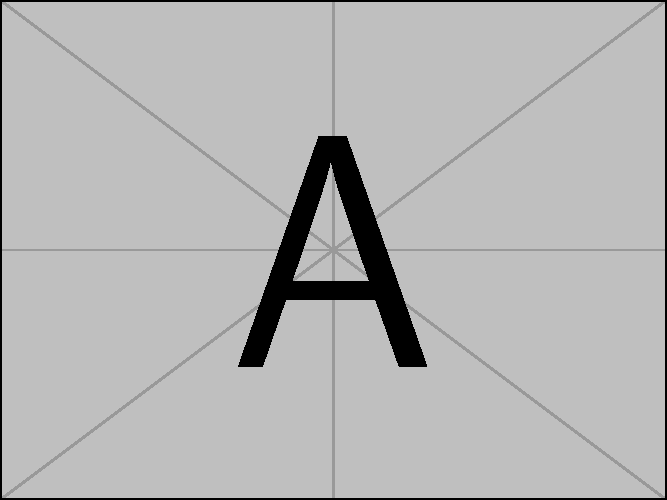
\includegraphics[width=.8\hsize]{figure/example-image-a.pdf} %
      \subcaption{Example Image A}
      \label{Fig:Example:A}
   \end{minipage}
   \begin{minipage}[b]{.3\hsize}
      \centering
      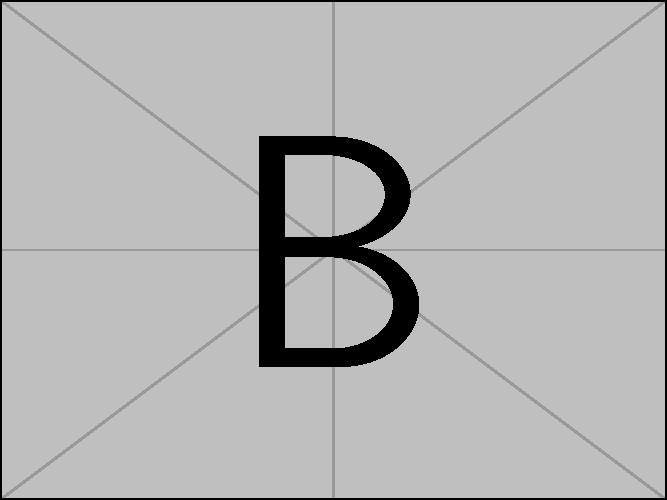
\includegraphics[width=.8\hsize]{figure/example-image-b.pdf} %
      \subcaption{Example Image B}
      \label{Fig:Example:B}
   \end{minipage}
   \begin{minipage}[b]{.3\hsize}
      \centering
      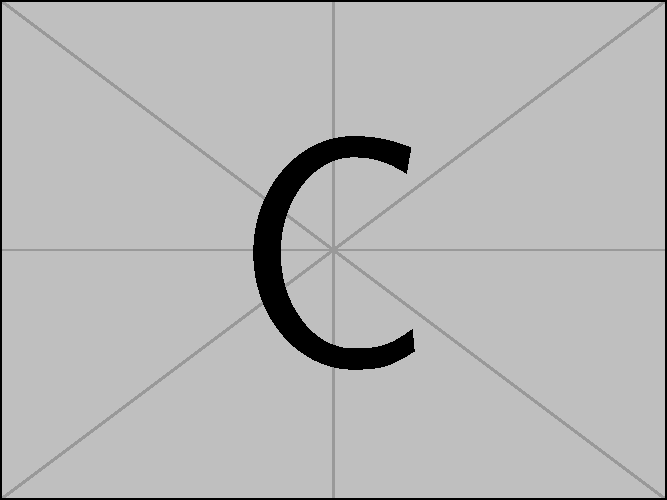
\includegraphics[width=.8\hsize]{figure/example-image-c.pdf} %
      \subcaption{Example Image C}
      \label{Fig:Example:C}
   \end{minipage}
   \caption{An Example of a Figure}
   \label{Fig:Example}
\end{figure*}

\lipsum[1]

\section{An Example of Floating Algorithm}
\lipsum[5-6]

%% アルゴリズム図を入れる方法
%% algorithmic マークアップの書き方は以下を参照
%%   http://mirrors.ctan.org/macros/latex/contrib/algorithms/algorithms.pdf
\begin{algorithm}[t]
   \caption{An Example of an Algorithm}
   \begin{algorithmic}[1]
      \REQUIRE $n\geq0$
      \ENSURE $y=x^n$
      \STATE $S\leftarrow0$
      \IF{Condition}
         \STATE Do something.
      \ELSE
         \STATE Do something.
      \ENDIF
      \FOR{$i=0$ \TO $10$}
         \STATE Carry out some processing.
      \ENDFOR
      \RETURN $S$
   \end{algorithmic}
\end{algorithm}

\lipsum[9-11]

\section{Something}
\lipsum[12-15]

%---------------------------------------------------------
% \balance コマンドを入れて最終ページの段組を揃える.
% 場所によってはうまく動作しないので適宜場所を調整する 
%  ・\bibliography の直前
%  ・Conclusion の節の直前
% など
\balance
%---------------------------------------------------------

\section{Conclusion}
\lipsum[4]

%% 謝辞は IEEE Conference では入れない
%\section*{Acknowledgment}

%% 参考文献リスト
\bibliography{IEEEexample,cites.bib}

\end{document}


